\chapter{Adattartományok a Calcban}
\thispagestyle{empty}

A Calc segítségével egyszerűbb adatbázis-funkciókat is
megvalósíthatunk. Az adatokat kötött formátumú
táblázatba kell beírnunk. Az ilyen táblázat oszlopai azonos
típusú adatokat tartalmaznak, az első sorba pedig az oszlopok
neveit kell beírni. A táblában az oszlopokat mezőknek, a
sorokat rekordoknak, az első sor adatait pedig mezőneveknek nevezzük. 
A táblában lehetőleg ne legyenek üres sorok vagy
oszlopok. Ezeknek a kritériumoknak megfelelnek a 18. feladatban
használt adatok. Másoljuk az A1:E17 tartományt az újonnan
létrehozott calc05 munkafüzet második munkalapjára (\ref{Adattartományok}
ábra). A munkalap neve legyen Adatok.

\begin{figure}[!h]
\begin{center}
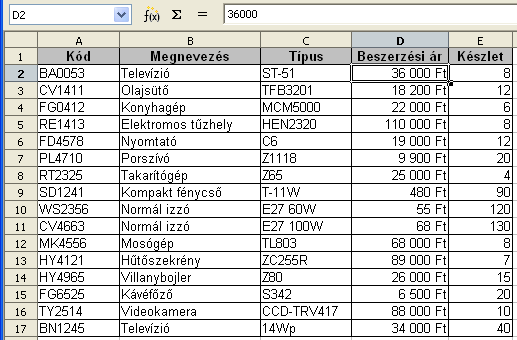
\includegraphics[width=13.679cm]{oocalcv2-img111.png}
\caption{Adattartományok}\label{Adattartományok}
\end{center}
\end{figure}

A táblában a következő mezőneveket látjuk: Kód,
Megnevezés, Típus, Beszerzési ár, Készlet. A tábla sorai
pedig a rekordok lesznek.


\section{Rendezés}

Calcban különböző szempontok szerint rendezhetjük
cellatartományok tartalmát. A \textbf{Standard} eszköztár
\textbf{Rendezés} \textbf{növekvő sorrendbe} és
\textbf{Csökkenő} \textbf{sorrend} parancsait csak akkor
használjuk, ha egy tartományt a mellette lévő
tartományoktól függetlenül akarunk rendezni. Olyan kötött
formátumú adattáblák rendezéséhez, mint amilyet \aref{Adattartományok}
ábrán is látunk, válasszuk a tábla egyik kitöltött
celláját és az \textbf{Adatok} menüpont \textbf{Rendezés}
parancsát (\ref{RendezésiFeltétel} ábra).

\begin{figure}[!h]
\begin{center}
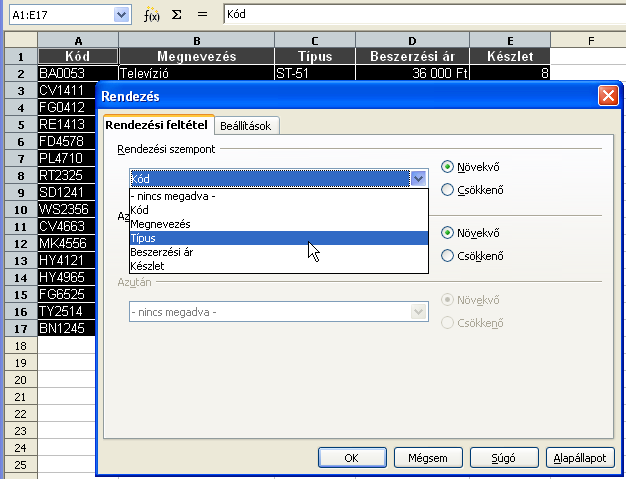
\includegraphics[width=15.999cm]{oocalcv2-img112.png}
\caption{Rendezés -- rendezési feltétel}\label{RendezésiFeltétel}
\end{center}
\end{figure}

Látjuk, hogy a Calc kijelölte az adattartományt. A megjelenő
párbeszédablakban kiválaszthatjuk azt a mezőt, amelyik
szerint rendezni szeretnénk adatainkat. Ismétlődő adatok
esetén lehet hasznos a másodlagos és a harmadlagos rendezés
beállítása. Mindhárom rendezésnél a rendezés irányát
is megadhatjuk.

A \textbf{Beállítások} fület választva (\ref{RendezésBeállítások} ábra)
megadhatjuk, hogy rendezésnél a kis- és nagybetűket
megkülönböztesse-e a program.

\begin{figure}[!h]
\begin{center}
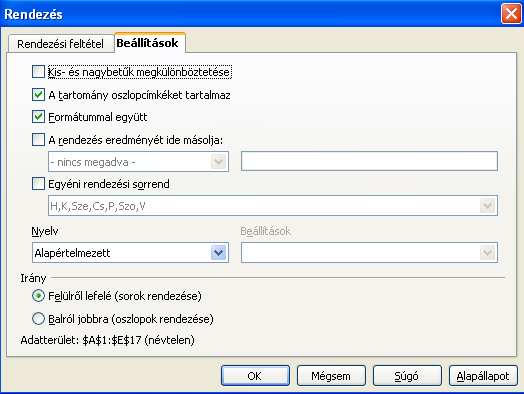
\includegraphics[width=12.864cm]{oocalcv2-img113.png}
\caption{Rendezés --  Beállítások}\label{RendezésBeállítások}
\end{center}
\end{figure}

\textbf{A tartomány oszlopcímeket tartalmaz} kapcsoló
meghatározza, hogy a mezőneveket, vagy az oszlopazonosítókat
használja az oszlopok azonosítására. Kikapcsolva az első
sort is rendezi a Calc. A rendezés eredményét egyszerűen
átmásolhatjuk egy névvel megadott cellatartományba, vagy
megadhatunk egy cellacímet, ahova a másolat bal felső
celláját helyezi. Ahhoz, hogy a Munkalap3 nevű munkalapon
jelenjen meg a táblázat másolata a beállított
rendezésekkel, a \textbf{Munkalap3.A1} címet kell beírnunk.


\section{Az automatikus szűrő használata}

A Calcban különböző szűréseket végezhetünk
adatainkon. Az adattartomány bármelyik cellájára kattintva, az
\textbf{Adat} menüpont \textbf{Szűrő} -- \textbf{Automatikus
szűrő} parancsával egy kombinált listát kapcsolhatunk be
a mezőnevek cellái mellett. Ezek valamelyikére kattintva
kiválaszthatunk egy elemet. Ilyenkor csak azok a rekordok jelennek
meg, amelyek eleget tesznek a szűrőfeltételben megadottnak.
\Aref{AutomatikusSzűrő} ábrán azokat a rekordokat mutatja
a szűrés eredménye, ahol a készlet értéke~8.

\begin{figure}[!h]
\begin{center}
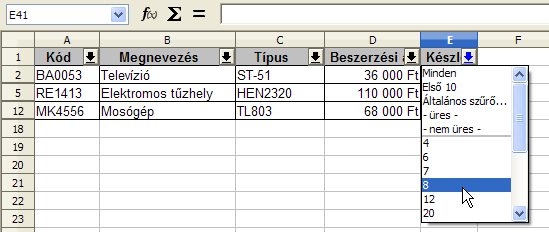
\includegraphics[width=13.524cm]{oocalcv2-img114.png}
\caption{Automatikus szűrő használata}\label{AutomatikusSzűrő}
\end{center}
\end{figure}

Az aktív szűrő oszlopában a nyílgomb kék színűre
vált. További szűrőket választva, a legördülő
listában már csak a szűrt adatok közül választhatunk. Az
aktív szűrőt a \textbf{minden} lehetőséget
választva kapcsolhatjuk ki.


\section{Általános szűrő}

Az \textbf{Adat} menüpont \textbf{Szűrő} --
\textbf{Általános} \textbf{szűrő} parancsával
meghatározhatunk bonyolultabb szűrési feltételeket (\ref{ÁltalánosSzűrő}
ábra).

\begin{figure}[!h]
\begin{center}
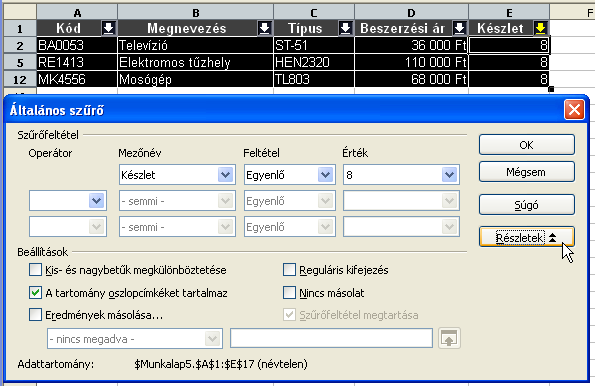
\includegraphics[width=13.743cm]{oocalcv2-img115.png}
\caption{Általános szűrő}\label{ÁltalánosSzűrő}
\end{center}
\end{figure}

Módosíthatjuk az automatikus szűrővel kiválasztott
feltételt, és meghatározhatunk még további kettőt. A
három szűrőfeltétel között ÉS vagy VAGY kapcsolat
lehet. A Részletek kapcsolóval bekapcsolhatjuk a kis- és
nagybetűk megkülönböztetését, a szűrt sorokat egy
másik helyre másolhatjuk, hasonlóképpen mint rendezésnél. A
\textbf{Reguláris kifejezés} bekapcsolásával
\textbf{Egyenlő} vagy \textbf{Nem egyenlő} feltétel esetén
az érték mezőbe reguláris kifejéseket is írhatunk. Ezek
részletes leírását az OpenOffice.org Calc Súgójában
megtaláljuk.


\section{25. feladat}

{\itshape
Szűrjük ki azokat a rekordokat az adattáblából amelyeknél
a típusnév Z betűvel kezdődik, a beszerzési ár pedig
10000 és 50000 közötti. Az E20 cellában függvénnyel
határozzuk meg a készletértékek összegét.}

Azt hogy egy szöveg Z betűvel kezdődik a
,,Z.*'' reguláris kifejezéssel
adhatjuk meg, hiszen a . (pont) bármilyen karaktert jelöl, a *
(csillag) pedig az előtte lévő karakter nulla vagy több
előfordulását. Egyszerre kell érvényesülnie a másik
két feltételnek is, tehát az ÉS kapcsolatot válasszuk a sorok
között (\ref{25-feladatÁltalános} ábra).

\begin{figure}[!h]
\begin{center}
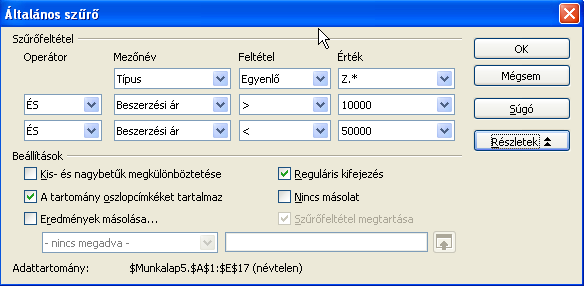
\includegraphics[width=13.452cm]{oocalcv2-img116.png}
\caption{25. feladat --  Általános szűrő}\label{25-feladatÁltalános}
\end{center}
\end{figure}

A szűrt rekordok értékeinek összegzésére nem
használhatjuk a SZUM függvényt, mert az tartalmazni fogja a
rejtett cellákban található értékeket is. A \textbf{Képlet}
eszköztár \textbf{Összeg} ikonjára kattintva a
\textbf{RÉSZÖSSZEG} függvény jelenik meg (\ref{25-feladatSUBTOTAL} ábra).

\begin{figure}[!h]
\begin{center}
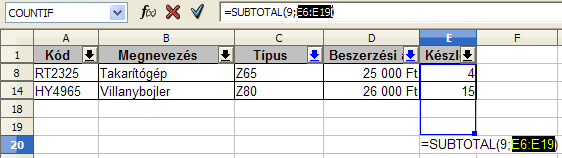
\includegraphics[width=13.868cm]{oocalcv2-img117.png}
\caption{25. feladat --  RÉSZÖSSZEG függvény}\label{25-feladatSUBTOTAL}
\end{center}
\end{figure}

Ez a függvény a szűrt eredményekkel végez
különböző műveleteket, amit az első paraméterében
megadott számmal határozunk meg. 9 a SZUM függvénynek felel meg.
A függvényindexek listáját megtaláljuk a Calc
súgójában.


\section{Irányított szűrés}

Az \textbf{Adat} menüpont \textbf{Szűrő} --
\textbf{Irányított szűrő} parancsával egy
szűrőfeltételeket tartalmazó cellatartomány alapján
végezhetünk szűrést az adattartományon.

\begin{figure}[!h]
\begin{center}
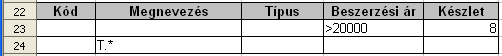
\includegraphics[width=12.282cm]{oocalcv2-img118.png}
\caption{Irányított szűrő}\label{IrányítottSzűrő}
\end{center}
\end{figure}

Készítsünk másolatot az adattáblánk mezőneveit
tartalmazó cellatartományról az A22:E22 tartományba. Az A22:E24
cellatartomány legyen szegélyezett. Az üres cellatartományba
írjunk különböző feltételeket (\ref{IrányítottSzűrő} ábra).

Ez a tartomány adja meg az irányított szűrő feltételeit.
Egy sor cellái között ÉS logikai kapcsolat lesz, a sorok
között pedig VAGY. \Aref{IrányítottSzűrő} ábrán látható feltételek azokat
a rekordokat határozzák meg, amelyekből 8 db van és a
beszerzési ár több mint 20000, és még minden olyan rekordot
amelyik megnevezése T betűvel kezdődik, függetlenül a
beszerzési ártól és darabszámtól.

Válasszuk az eredeti adattartomány valamelyik celláját és
az \textbf{Adat} menüpont \textbf{Szűrő} --
\textbf{Irányított szűrő} parancsát. A megjelenő
ablakban adjuk meg szűrőfeltételnek az A22:E24 tartományt,
és kapcsoljuk be a Reguláris kifejezések kapcsolót, hiszen a
B24 cellába ilyet írtunk. A megjelenő, a feltételeknek
megfelelő szűrt tartományt \aref{SzűrésEredmények} ábra mutatja.

\begin{figure}[!h]
\begin{center}
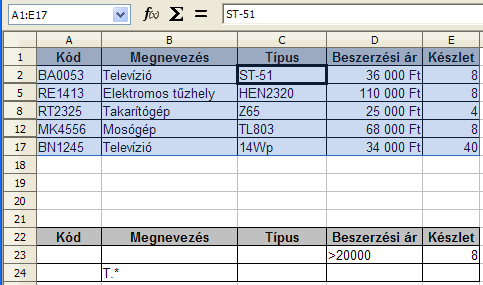
\includegraphics[width=12.778cm]{oocalcv2-img119.png}
\caption{Szűrés eredmények}\label{SzűrésEredmények}
\end{center}
\end{figure}

A szűrőfeltételek módosítása után azok automatikusan
nem jutnak érvényre. A szűrés aktualizálásához
ismételten ki kell adni az \textbf{Adat} menüpont
\textbf{Szűrő -- Irányított szűrő} parancsát.

